\section{Characterization of QCS}

\subsection{Quantum Circuit Benchmarks}
\label{sec:bench}
\begin{table}[t!]
    \centering
    %\scriptsize
        \caption{List of quantum circuit benchmarks.}
    \begin{tabular}{||c|c||}
        \hline
        {\bf Abbrv.} & {\bf Application} \\
        [0.5ex] 
        \hline\hline
        {\tt hchain} & Linear hydrogen atom chain \cite{10.1021/acs.jctc.9b01125} \\
        \hline
        {\tt rqc} & Random quantum circuit \cite{10.1038/s41567-018-0124-x} \\
        \hline
        {\tt qaoa} & Quantum approximate optimization algorithm \cite{10.48550/arXiv.1411.4028}  \\
        \hline
        {\tt gs} & Graph state \cite{10.26421/QIC17.3-4-5,10.3254/978-1-61499-018-5-115} \\
        \hline
        {\tt hlf} & Hidden linear function \cite{10.1126/science.aar3106} \\
        \hline
        {\tt qft} & Quantum Fourier transform \cite{10.1016/j.parco.2014.12.001} \\
        \hline
        {\tt iqp} & Instantaneous quantum polynomial-time \cite{10.1098/rspa.2010.0301,10.1103/PhysRevLett.117.080501} \\
        \hline
        {\tt qf} & Quadratic form \cite{10.22331/q-2021-04-08-428} \\
        \hline
    \end{tabular}
    \label{tab:list-bench}
\end{table}

In this paper, we characterize the performance of QCS using a rich set of quantum circuits. Table \ref{tab:list-bench} lists the circuit benchmarks. 
\begin{itemize}
\item {\tt hchain:}
This circuit which describes a system of hydrogen atoms arranged linearly is a representative quantum chemistry application\cite{10.1103/PhysRevX.10.031058,10.1063/1.2770707,10.1063/1.2345196,10.1063/1.5129672,10.1103/PhysRevA.95.020501}. This circuit incorporates increased circuit depth and an early entanglement in terms of total operations.
\item {\tt rqc:}
The random quantum circuit from Google \cite{10.1038/s41567-018-0124-x,10.1038/s41567-018-0318-2} is used to represent the quantum supremacy compared to classical computers. 
\item {\tt qaoa:} 
Quantum approximate optimization is a promising quantum algorithm in the NISQ era that produces approximate solutions for combinatorial optimization problems \cite{10.48550/arXiv.1411.4028}. 
\item {\tt gs:}
This circuit is used to prepare graph states \cite{10.1103/PhysRevA.71.012319} that are multi-particle entangled states. Examples include many-body spin states of distributed quantum systems that are important in quantum error correction \cite{10.1017/CBO9781139034807}. 
\item {\tt hlf:}
This benchmark circuit solves the 2D hidden linear function problem \cite{10.1126/science.aar3106}. 
\item {\tt qft:}
The quantum Fourier transform circuit \cite{10.1016/j.parco.2014.12.001} is the quantum analog of the inverse discrete Fourier transform. It is an important function in Shor's algorithm \cite{10.1137/S0036144598347011}.
\item {\tt iqp:} 
The instantaneous quantum polynomial circuit provides evidence that sampling the output probability distribution of a quantum circuit is difficult when using classical approaches \cite{10.1098/rspa.2010.0301,10.1103/PhysRevLett.117.080501}.
\item {\tt qf:}
This circuit implements a quadratic form on binary variables encoded in qubit registers. It is used to solve the quadratic unconstrained binary optimization problems \cite{10.22331/q-2021-04-08-428}.
\end{itemize}

\subsection{Baseline QCS}
\label{sec:baseline}
In this paper, we use the popular IBM QISKit-Aer simulator. We consider the state-of-the-art GPU-supported simulation~\cite{10.1145/3310273.3323053} in QISKit-Aer as our baseline. We run all simulations on a server with dual 10-core Intel Xeon Silver 4114 CPUs at 2.2 GHz, 384 GB of memory, and an NVIDIA P100 GPU with 16 GB of memory connected through PCI-e\footnote{We used the P100 GPU as the HPC platform to test and evaluated the proposed Q-GPU. It is important to emphasize that our approach is not bound to P100. Our proposed Q-GPU is applicable to any other GPU architectures.}. We use CUDA v10 and Nvprof~\cite{NVIDIAnvprof} to conduct our characterization. The simulation in QISKit-Aer has three key steps: 1) state vector partitioning, 2) static state amplitudes allocation, and 3) on-demand amplitudes exchange. 

\noindent\textbf{Step 1: State vector partitioning:} QISKit-Aer first partitions the state vectors into "chunks". Chunk is the granularity used in the simulator to update the state vector. For illustrative purposes, let us assume we have a 7-qubit circuit, i.e., that there are in total $2^7$ different state amplitudes from $a_{0000000}$ to $a_{1111111}$. All the states are stored in a vector (i.e., the state vector), and this state vector is partitioned into chunks. For example, assuming we divide the state vector into 8 chunks, each chunk contains 16 state amplitudes as shown in Figure~\ref{fig-3}. The three most significant bits are used to index the chunks, and the remaining bits are as offsets within a chunk.

\noindent\textbf{Step 2: Static chunk allocation:} After partitioning, these chunks are allocated into GPU memory based on the GPU memory availability. As illustrated in Figure~\ref{fig-3}, if a GPU can only store 3 chunks, the remaining 5 chunks will be stored in the host CPU memory. For example, when 64 GB memory is needed to simulate 32 qubits, the first 16 GB is allocated in GPU memory (in P100 GPU with 16 GB memory) and the remaining 48 GB is in the CPU memory. 

\noindent\textbf{Step 3: Reactive chunk exchange:} During circuit simulation, a chunk exchange between the GPU and the CPU arises when the requested state amplitudes are not locally available on the GPU. In QISKit-Aer, the chunk exchange between the CPU and the GPU is triggered on-demand. That is, when both the chunks on the CPU and the GPU are involved in one state-update calculation, the corresponding CPU chunks are transferred to GPU for updating. After the operation, the updated chunks are transferred back to the CPU. Note that, the amount of data exchange in the following scenarios is dependent on the qubits in the specific gate simulation.

\begin{itemize}
\item \textbf{Case 1: All the indices of the qubits involved in the current gate are smaller than the chunk size:}. For example, a gate on qubit $0$ requires amplitudes $a_{\times\times\times\times\times\times\times0}$ and $a_{\times\times\times\times\times\times\times1}$ 
(see Equation~\ref{eq:amplituesupdate}). In this case,  each chunk can be updated independently without requiring extra data movement. 

\item \textbf{Case 2: Some indices of qubits involved in the current gate are outside the chunk boundary:} In this scenario, let us assume there is a gate that operates on $q_6$, thereby the required pairs of amplitudes are $a_{\times0\times\times\times\times\times\times}$ and $a_{\times1\times\times\times\times\times\times}$. However, as depicted in Figure~\ref{fig-3}, none of the chunks contains a pair of required amplitudes, i.e., the computation for updating amplitudes involves more than one chunk. 
Specifically, to update the pairs of amplitudes, we need ($chunk_0$, $chunk_2$), ($chunk_1$, $chunk_3$), $\dots$, and ($chunk_5$, $chunk_7$). However, ($chunk_1$, $chunk_3$) involves one chunk on the GPU and one chunk on the CPU. In this scenario, data exchange is required. 
In the baseline QISKit-Aer simulation, the requested chunks are always copied from CPU to GPU. That is, in the example above, the CPU copies $chunk_3$ to GPU. After the $chunk_3$ is updated together with $chunk_1$, it is copied back to the CPU memory. 

\end{itemize}

Note that, as the GPU memory capacity is much less compared to the CPU host memory, a large number of chunks are statically allocated on CPU memory when the number of qubits is large. For instance, on the P100 GPU with 16 GB memory, we observe from experiments that when simulating a circuit that has 34 qubits, the state vector is divided into 8192 chunks, 496 chunks are allocated on GPU, while the remaining 7696 chunks are all on CPU. Therefore, one can expect that most of the time, the CPU does the state amplitude update without benefiting from the GPU acceleration. 

\begin{figure}[h!]
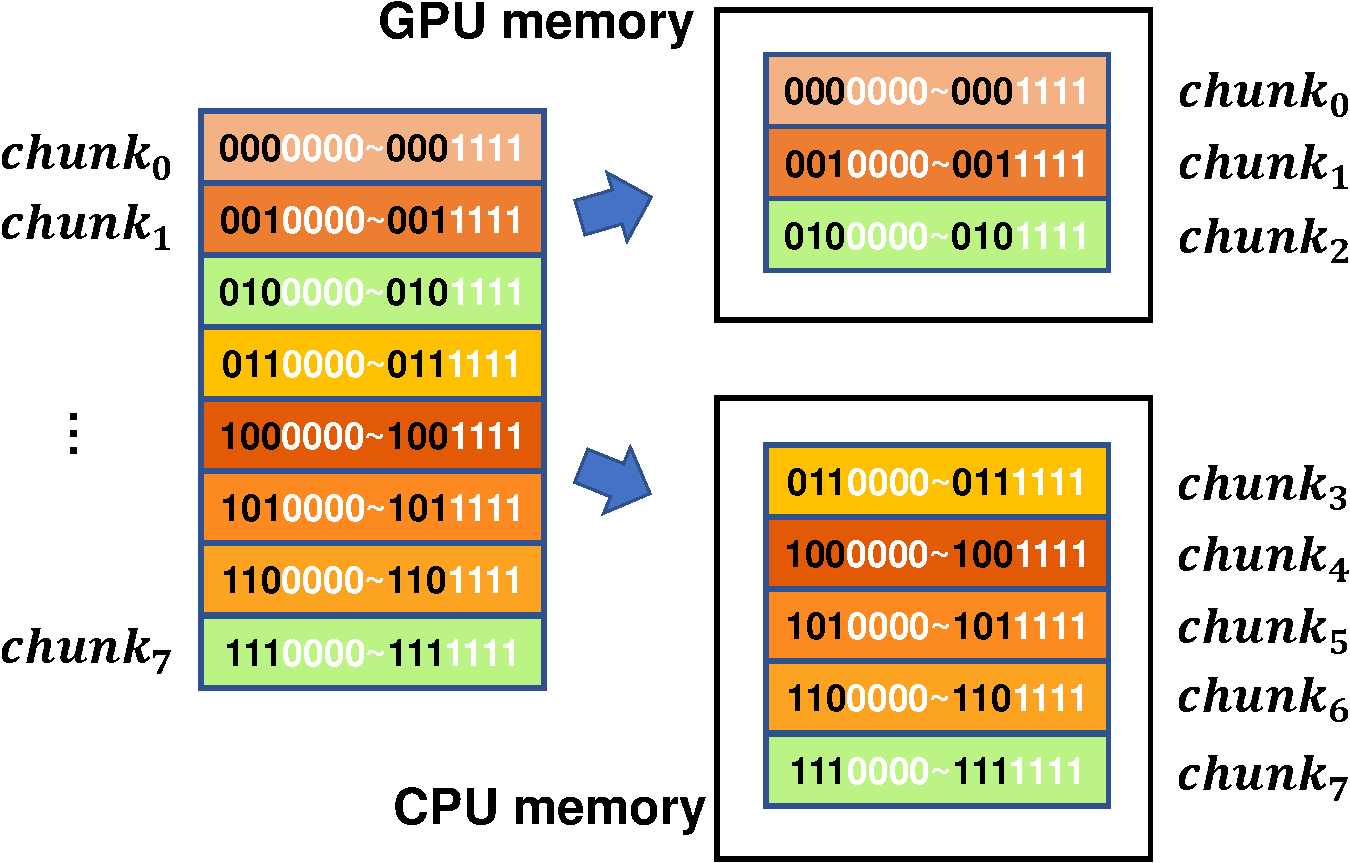
\includegraphics[width=\textwidth]{Images/appendix2/section-3/chunk-egs.pdf}
\centering
\caption{Example of baseline execution where the state vector is statically partitioned and allocated on CPU and GPU.} %\xulong{update to be more space efficient}}
\label{fig-3}
\vspace{-5pt}
\end{figure}

\subsection{Characterization and Observations}
\label{sec:observation}

In this section, we quantify the simulation performance of the baseline QISKit-Aer.
We first study the scalability when the number of qubits increases. We observe that, if there are less than 30 qubits in the circuit, the baseline GPU simulates much faster than compared CPU-based simulation (e.g. 9.67$\times$ speedup for 29-qubit circuits on average), since the entire state vector fits in the P100 GPU memory and there is no need for data exchange and synchronization. However, the baseline GPU performance significantly drops when the number of qubits is larger than 30. It becomes even worse than running on the CPU alone when the number of qubits reaches 32. In particular, we observe a factor of $1.8\times$ slowdown for {\tt qft\_33}\footnote{In this paper, we use $n$ in the circuit name (e.g., {\tt circ\_n}) to represent a circuit with $n$ qubits.} as an example. 

\begin{figure}[h!]
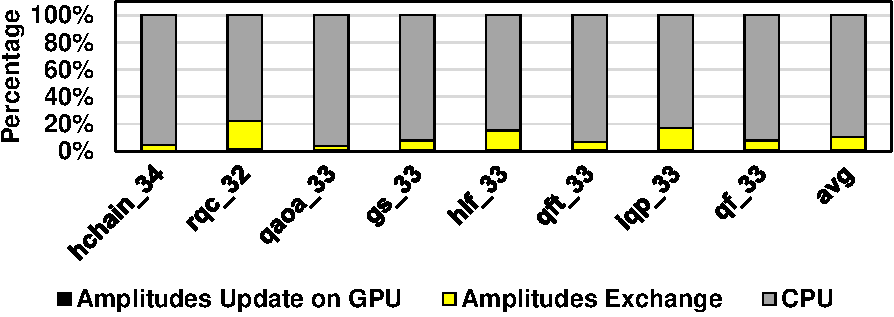
\includegraphics[width=\textwidth]{Images/appendix2/section-3/baseline-breakdown.pdf}
\caption{Baseline execution time breakdown.}
\label{fig:basebreak}
\vspace{-5pt}
\end{figure}

To investigate the reason for this slowdown, we show the breakdown of the execution time in Figure \ref{fig:basebreak}. One can observe that, on average, 89.34\%  of the execution is spent on the CPU, indicating that the GPUs are not properly used in the baseline execution for large number qubit circuits. Moreover, the overheads involve amplitude exchange and synchronization occupies 9.91\% of the average execution time, and the computation time of GPU only occupies 0.71\% of total time on average. \emph{In other words, most of the computation is performed by the CPU and the GPU is idle due to the static state chunk allocation in the baseline GPU execution.} In Figure \ref{fig:timeline-overlap}, \circledwhite{I} depicts the execution timeline of the baseline.

%%%%%%%%%%%%%%%%%%%%%%%%

\subsection{Will a Naive Optimization Work?}
\label{sec:naive}
To improve the GPU utilization during simulation, an intuitive optimization would dynamically allocate the chunks and transfer the chunks to GPU for updates. In this section, we investigate whether the naive implementation works well or not.
\begin{figure}[!h]
    \centering
    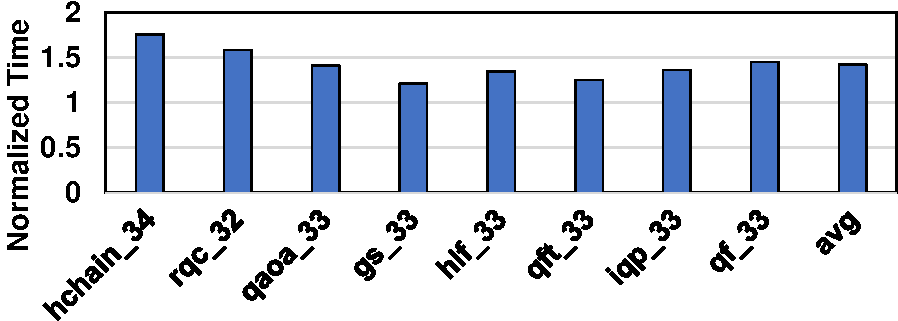
\includegraphics[width=\textwidth]{Images/appendix2/section-3/naive-base.pdf}
    \caption{Normalized execution time of naive approach.}
    \label{fig:naivebase}
    \vspace{-5pt}
\end{figure}

\begin{figure}[!h]
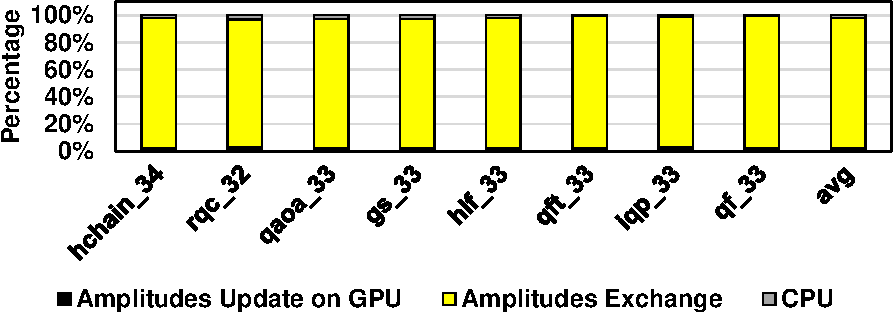
\includegraphics[width=\textwidth]{Images/appendix2/section-3/naive.pdf}
\centering
\caption{Execution time breakdown of naive optimization.} 
\label{fig:naivebreak}
\end{figure}

We implemented the dynamic state vector chunk allocation in QISKit-Aer. Figure \ref{fig:naivebase} depicts the execution time of the naive optimization normalized to the baseline execution. Surprisingly, none of the quantum circuits we studied show improvements when using dynamic allocation. To further investigate the reason, we break down the execution time and show the results in Figure~\ref{fig:naivebreak}.
As can be seen from the figure, while CPU execution time significantly reduces and the data movement dominates, indicating that the GPU is waiting for data most of the time during execution.
Therefore, naive dynamic allocation alone does not work to deliver good QCS performance. More sophisticated end-to-end optimizations are required to systematically improve the QCS performance and scalability. 

